\documentclass{beamer}


\usepackage[utf8]{inputenc}
\usepackage{lmodern} 
\usepackage[utf8]{inputenc}
\usepackage{lmodern} 
\usepackage{listings}
\usepackage{xcolor} 
\usepackage{graphicx}

\lstset{
	language=C,
	basicstyle=\ttfamily\small,
	keywordstyle=\color{blue},
	commentstyle=\color{green},
	stringstyle=\color{red},
	breaklines=true,
	breakatwhitespace=true,
	showstringspaces=false,
	frame=single,
	morekeywords={import, as, from, ctypes, numpy, matplotlib, pyplot, None},
	xleftmargin=0pt,
	framexleftmargin=0pt,
	aboveskip=0pt,
	belowskip=0pt
}




\definecolor{myblue}{RGB}{48, 63, 159}

\setbeamercolor{palette primary}{bg=myblue, fg=white}
\setbeamercolor{structure}{fg=myblue}
\setbeamercolor{frametitle}{bg=myblue, fg=white}
\setbeamercolor{title}{bg=myblue, fg=white}
\setbeamercolor{footlinecolor}{bg=myblue, fg=white}


\defbeamertemplate*{title page}{mytemplate}{
	\vfill
	\begin{center}

		\begin{beamercolorbox}[wd=0.8\paperwidth, center, rounded=true, shadow=true]{title}
			\usebeamerfont{title}\inserttitle\par
		\end{beamercolorbox}
		\vspace{2cm} 

		\usebeamerfont{author}\insertauthor
		\vspace{1cm} 
		\usebeamerfont{date}\insertdate
	\end{center}
	\vfill
}


\defbeamertemplate*{frametitle}{mytemplate}{
	\begin{beamercolorbox}[wd=\paperwidth, ht=2.5ex, dp=1.5ex, left]{frametitle}
		\hspace{1em}\usebeamerfont{frametitle}\insertframetitle
	\end{beamercolorbox}
}


\setbeamertemplate{footline}{
	\begin{beamercolorbox}[wd=\paperwidth, ht=2.25ex, dp=1ex]{footlinecolor}
		\hspace{1em}\usebeamerfont{author in footline}\insertshortauthor
		\hfill
		\usebeamerfont{title in footline}\insertshorttitle
		\hfill
		\usebeamerfont{date in footline}\insertdate \hspace{1em} \insertframenumber/\inserttotalframenumber \hspace{0.5em}
	\end{beamercolorbox}
}


\setbeamerfont{author in footline}{size=\tiny}
\setbeamerfont{title in footline}{size=\tiny}
\setbeamerfont{date in footline}{size=\tiny}



\title{4.11.30}
\author{Shriyansh Chawda-EE25BTECH11052}
\date{August 23, 2025}



\begin{document}
	

		\setbeamertemplate{footline}{} 
		\frame{\titlepage}
	
	
	\begin{frame}{Question} 
Draw the graph of the equations $x - y + 1 = 0$ and $3x + 2y - 12 = 0$. Using this graph, find the values of $x$ and $y$ which satisfy both the equations. 
		\hfill (10, 2021)
	\end{frame}
	

\begin{frame}{Solution}
	Below is the Graph plotted for the given two lines.\\
	The lines intersect at (2,3).\\
\[
\begin{aligned}
	&\text{Given } 
	\begin{cases}
		x - y + 1 = 0\\
		3x + 2y - 12 = 0
	\end{cases}
	\;\Longleftrightarrow\;
	\begin{cases}
		x - y = -1\\
		3x + 2y = 12
	\end{cases} \\[4pt]
	&\text{Matrix form:}\quad
	\underbrace{\begin{bmatrix}1 & -1\\ 3 & 2\end{bmatrix}}_{A}
	\underbrace{\begin{bmatrix}x\\y\end{bmatrix}}_{\mathbf{x}}
	=
	\underbrace{\begin{bmatrix}-1\\12\end{bmatrix}}_{\mathbf{b}}.
\end{aligned}
\]
\end{frame}
\begin{frame}{Solution}
	\resizebox{\textwidth}{!}{$
		\left[ A \mid \mathbf{b} \right]
		=
		\left[
		\begin{array}{cc|c}
			1 & -1 & -1 \\
			3 & 2  & 12
		\end{array}
		\right]
		\xrightarrow{R_2 \leftarrow R_2 - 3R_1}
		\left[
		\begin{array}{cc|c}
			1 & -1 & -1 \\
			0 & 5  & 15
		\end{array}
		\right]
		\xrightarrow{R_2 \leftarrow \tfrac{1}{5}R_2}
		\left[
		\begin{array}{cc|c}
			1 & -1 & -1 \\
			0 & 1  & 3
		\end{array}
		\right]$}
		\[
		\;\xrightarrow{\,R_1 \leftarrow R_1 + R_2\,}\;
		\left[
		\begin{array}{cc|c}
			1 & 0 & 2\\
			0 & 1 & 3
		\end{array}
		\right]
		\;\Longrightarrow\;
		x = 2, y = 3.
		\]
\end{frame}

\begin{frame}{Graph}	
	\begin{figure}
		\centering
		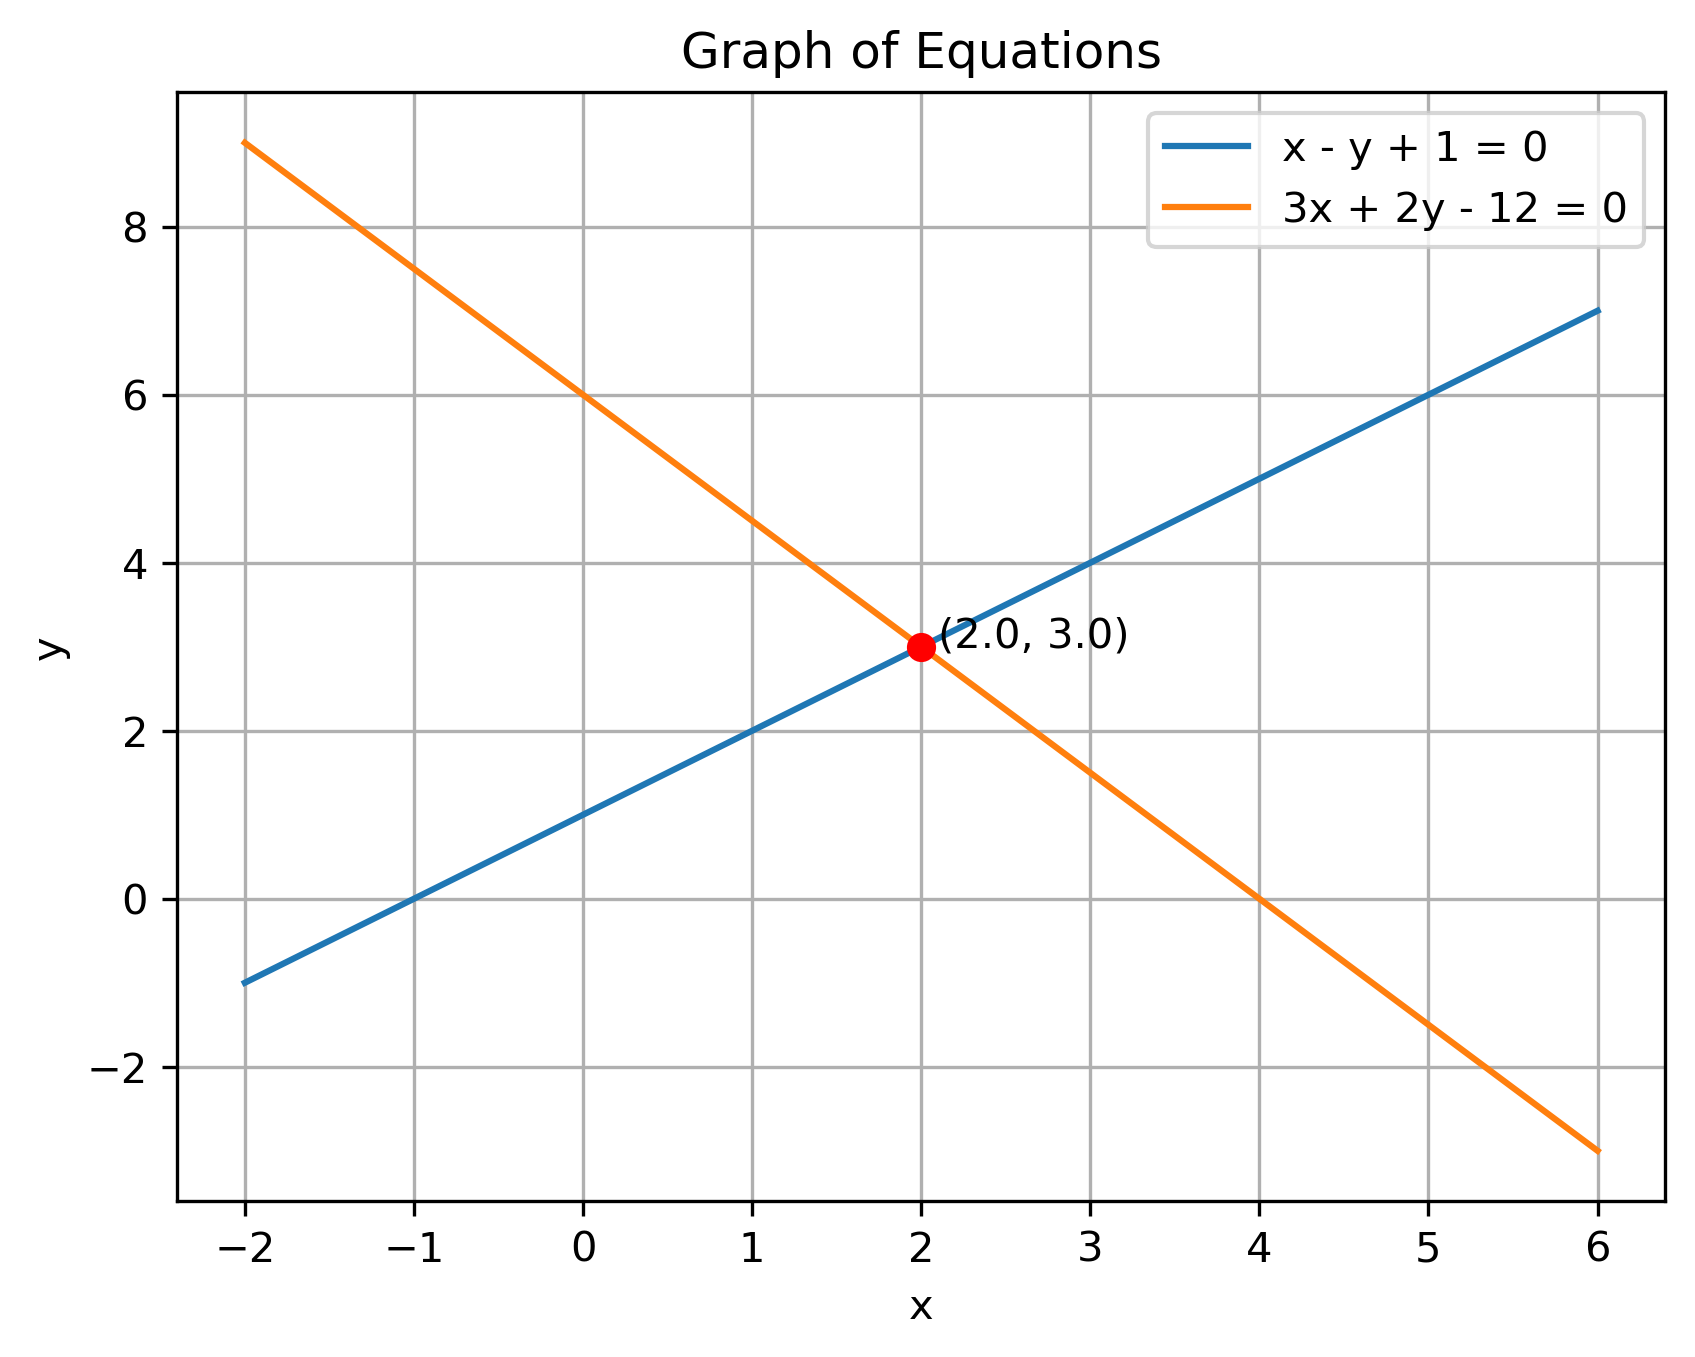
\includegraphics[width=0.8\linewidth]{figs/equations_solution}
		\label{fig:equationssolution}
	\end{figure}
	
	
\end{frame}



\end{document}